% Options for packages loaded elsewhere
% Options for packages loaded elsewhere
\PassOptionsToPackage{unicode}{hyperref}
\PassOptionsToPackage{hyphens}{url}
\PassOptionsToPackage{dvipsnames,svgnames,x11names}{xcolor}
%
\documentclass[
  letterpaper,
  DIV=11,
  numbers=noendperiod]{scrreprt}
\usepackage{xcolor}
\usepackage{amsmath,amssymb}
\setcounter{secnumdepth}{5}
\usepackage{iftex}
\ifPDFTeX
  \usepackage[T1]{fontenc}
  \usepackage[utf8]{inputenc}
  \usepackage{textcomp} % provide euro and other symbols
\else % if luatex or xetex
  \usepackage{unicode-math} % this also loads fontspec
  \defaultfontfeatures{Scale=MatchLowercase}
  \defaultfontfeatures[\rmfamily]{Ligatures=TeX,Scale=1}
\fi
\usepackage{lmodern}
\ifPDFTeX\else
  % xetex/luatex font selection
\fi
% Use upquote if available, for straight quotes in verbatim environments
\IfFileExists{upquote.sty}{\usepackage{upquote}}{}
\IfFileExists{microtype.sty}{% use microtype if available
  \usepackage[]{microtype}
  \UseMicrotypeSet[protrusion]{basicmath} % disable protrusion for tt fonts
}{}
\makeatletter
\@ifundefined{KOMAClassName}{% if non-KOMA class
  \IfFileExists{parskip.sty}{%
    \usepackage{parskip}
  }{% else
    \setlength{\parindent}{0pt}
    \setlength{\parskip}{6pt plus 2pt minus 1pt}}
}{% if KOMA class
  \KOMAoptions{parskip=half}}
\makeatother
% Make \paragraph and \subparagraph free-standing
\makeatletter
\ifx\paragraph\undefined\else
  \let\oldparagraph\paragraph
  \renewcommand{\paragraph}{
    \@ifstar
      \xxxParagraphStar
      \xxxParagraphNoStar
  }
  \newcommand{\xxxParagraphStar}[1]{\oldparagraph*{#1}\mbox{}}
  \newcommand{\xxxParagraphNoStar}[1]{\oldparagraph{#1}\mbox{}}
\fi
\ifx\subparagraph\undefined\else
  \let\oldsubparagraph\subparagraph
  \renewcommand{\subparagraph}{
    \@ifstar
      \xxxSubParagraphStar
      \xxxSubParagraphNoStar
  }
  \newcommand{\xxxSubParagraphStar}[1]{\oldsubparagraph*{#1}\mbox{}}
  \newcommand{\xxxSubParagraphNoStar}[1]{\oldsubparagraph{#1}\mbox{}}
\fi
\makeatother


\usepackage{longtable,booktabs,array}
\usepackage{calc} % for calculating minipage widths
% Correct order of tables after \paragraph or \subparagraph
\usepackage{etoolbox}
\makeatletter
\patchcmd\longtable{\par}{\if@noskipsec\mbox{}\fi\par}{}{}
\makeatother
% Allow footnotes in longtable head/foot
\IfFileExists{footnotehyper.sty}{\usepackage{footnotehyper}}{\usepackage{footnote}}
\makesavenoteenv{longtable}
\usepackage{graphicx}
\makeatletter
\newsavebox\pandoc@box
\newcommand*\pandocbounded[1]{% scales image to fit in text height/width
  \sbox\pandoc@box{#1}%
  \Gscale@div\@tempa{\textheight}{\dimexpr\ht\pandoc@box+\dp\pandoc@box\relax}%
  \Gscale@div\@tempb{\linewidth}{\wd\pandoc@box}%
  \ifdim\@tempb\p@<\@tempa\p@\let\@tempa\@tempb\fi% select the smaller of both
  \ifdim\@tempa\p@<\p@\scalebox{\@tempa}{\usebox\pandoc@box}%
  \else\usebox{\pandoc@box}%
  \fi%
}
% Set default figure placement to htbp
\def\fps@figure{htbp}
\makeatother





\setlength{\emergencystretch}{3em} % prevent overfull lines

\providecommand{\tightlist}{%
  \setlength{\itemsep}{0pt}\setlength{\parskip}{0pt}}



 


\KOMAoption{captions}{tableheading}
\makeatletter
\@ifpackageloaded{bookmark}{}{\usepackage{bookmark}}
\makeatother
\makeatletter
\@ifpackageloaded{caption}{}{\usepackage{caption}}
\AtBeginDocument{%
\ifdefined\contentsname
  \renewcommand*\contentsname{Table of contents}
\else
  \newcommand\contentsname{Table of contents}
\fi
\ifdefined\listfigurename
  \renewcommand*\listfigurename{List of Figures}
\else
  \newcommand\listfigurename{List of Figures}
\fi
\ifdefined\listtablename
  \renewcommand*\listtablename{List of Tables}
\else
  \newcommand\listtablename{List of Tables}
\fi
\ifdefined\figurename
  \renewcommand*\figurename{Figure}
\else
  \newcommand\figurename{Figure}
\fi
\ifdefined\tablename
  \renewcommand*\tablename{Table}
\else
  \newcommand\tablename{Table}
\fi
}
\@ifpackageloaded{float}{}{\usepackage{float}}
\floatstyle{ruled}
\@ifundefined{c@chapter}{\newfloat{codelisting}{h}{lop}}{\newfloat{codelisting}{h}{lop}[chapter]}
\floatname{codelisting}{Listing}
\newcommand*\listoflistings{\listof{codelisting}{List of Listings}}
\makeatother
\makeatletter
\makeatother
\makeatletter
\@ifpackageloaded{caption}{}{\usepackage{caption}}
\@ifpackageloaded{subcaption}{}{\usepackage{subcaption}}
\makeatother
\usepackage{bookmark}
\IfFileExists{xurl.sty}{\usepackage{xurl}}{} % add URL line breaks if available
\urlstyle{same}
\hypersetup{
  pdftitle={Riantama Putra},
  pdfauthor={18224061 Riantama Putra},
  colorlinks=true,
  linkcolor={blue},
  filecolor={Maroon},
  citecolor={Blue},
  urlcolor={Blue},
  pdfcreator={LaTeX via pandoc}}


\title{Riantama Putra}
\usepackage{etoolbox}
\makeatletter
\providecommand{\subtitle}[1]{% add subtitle to \maketitle
  \apptocmd{\@title}{\par {\large #1 \par}}{}{}
}
\makeatother
\subtitle{Portfolio Asesmen II-2100 KIPP}
\author{18224061 Riantama Putra}
\date{2025-10-22}
\begin{document}
\maketitle

\renewcommand*\contentsname{Table of contents}
{
\hypersetup{linkcolor=}
\setcounter{tocdepth}{2}
\tableofcontents
}

\bookmarksetup{startatroot}

\chapter*{Hello, World!}\label{hello-world}
\addcontentsline{toc}{chapter}{Hello, World!}

\markboth{Hello, World!}{Hello, World!}

\begin{figure}[H]

{\centering 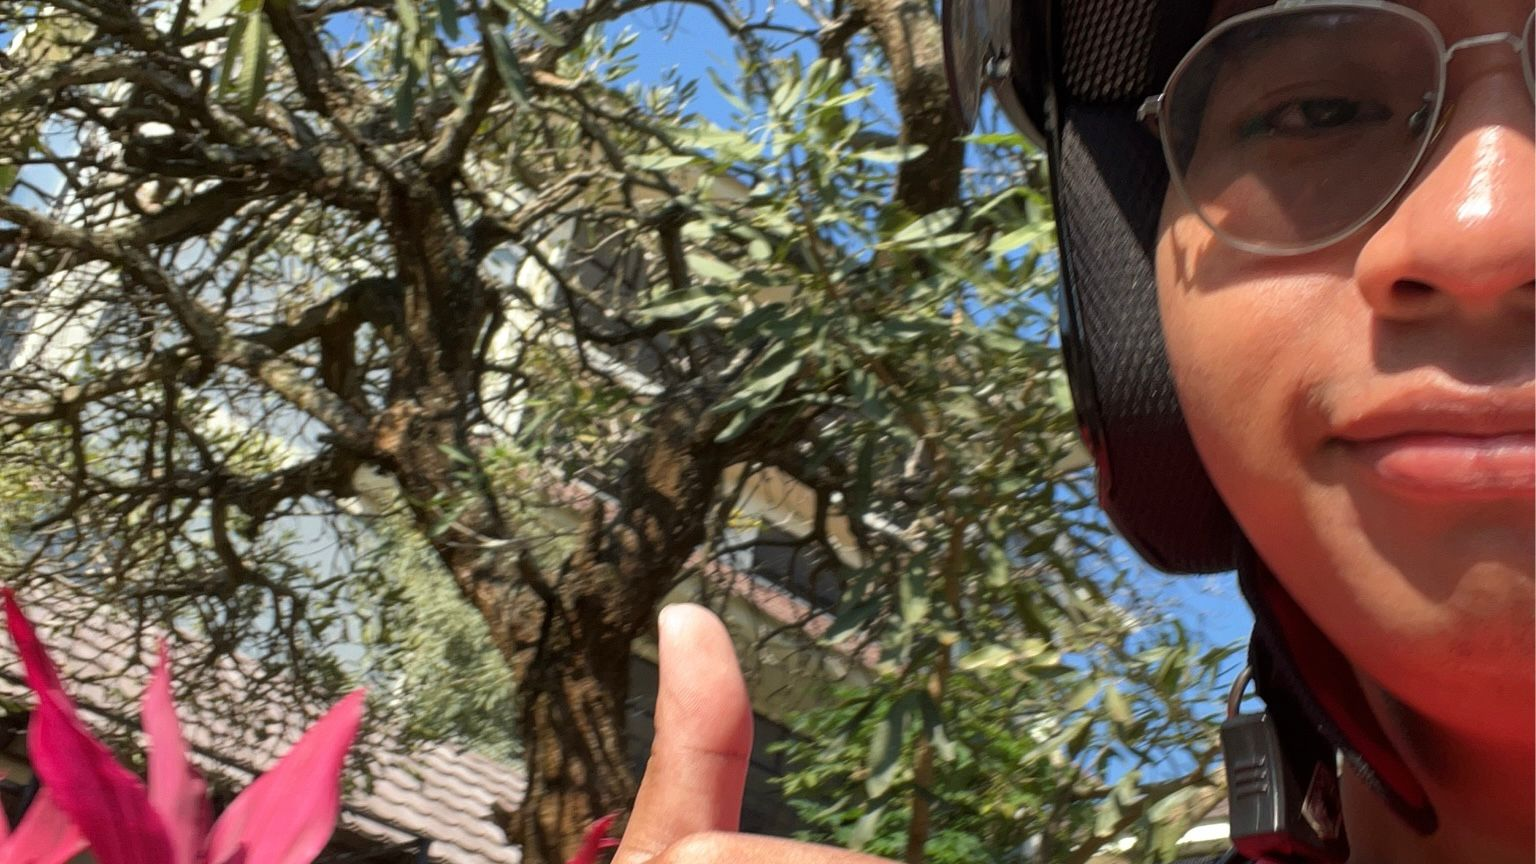
\includegraphics[width=9.5\linewidth,height=\textheight,keepaspectratio]{images/rian.jpeg}

}

\caption{Kenalan Dikit}

\end{figure}%

Perkenalkan Rian! Mahasiswa ITB, Sistem dan Teknologi Informasi Angkatan
2024.\\
Website ini dibuat sebagai bagian dari pemenuhan nilai Ujian Tengah
Semester mata kuliah Komunikasi Interpersonal dan Publik (II2100).

Tujuan utama dari situs ini adalah untuk menampilkan refleksi dan hasil
pembelajaran saya selama mengikuti mata kuliah ini, mulai dari pemahaman
diri dan komunikasi antarpribadi, hingga bagaimana konsep-konsep
tersebut diterapkan dalam kehidupan akademik dan profesional.

Di dalam website ini, Anda akan menemukan lima bagian utama yang
mewakili setiap topik penilaian UTS:

\begin{itemize}
\tightlist
\item
  \textbf{UTS-1:} All About Me\\
\item
  \textbf{UTS-2:} My Songs for You\\
\item
  \textbf{UTS-3:} My Stories for You\\
\item
  \textbf{UTS-4:} My SHAPE (Spiritual Gifts, Heart, Abilities,
  Personality, Experiences)\\
\item
  \textbf{UTS-5:} My Personal Reviews
\end{itemize}

Saya berharap melalui portofolio ini, Anda dapat melihat proses saya
dalam memahami, mengevaluasi, dan mengembangkan keterampilan komunikasi
yang lebih efektif. Baik dalam konteks pribadi, akademik, maupun sosial.

Atur-atur sendiri lah ya :\textgreater{}

\bookmarksetup{startatroot}

\chapter{UTS-1 All About Me}\label{uts-1-all-about-me}

\begin{figure}[H]

{\centering 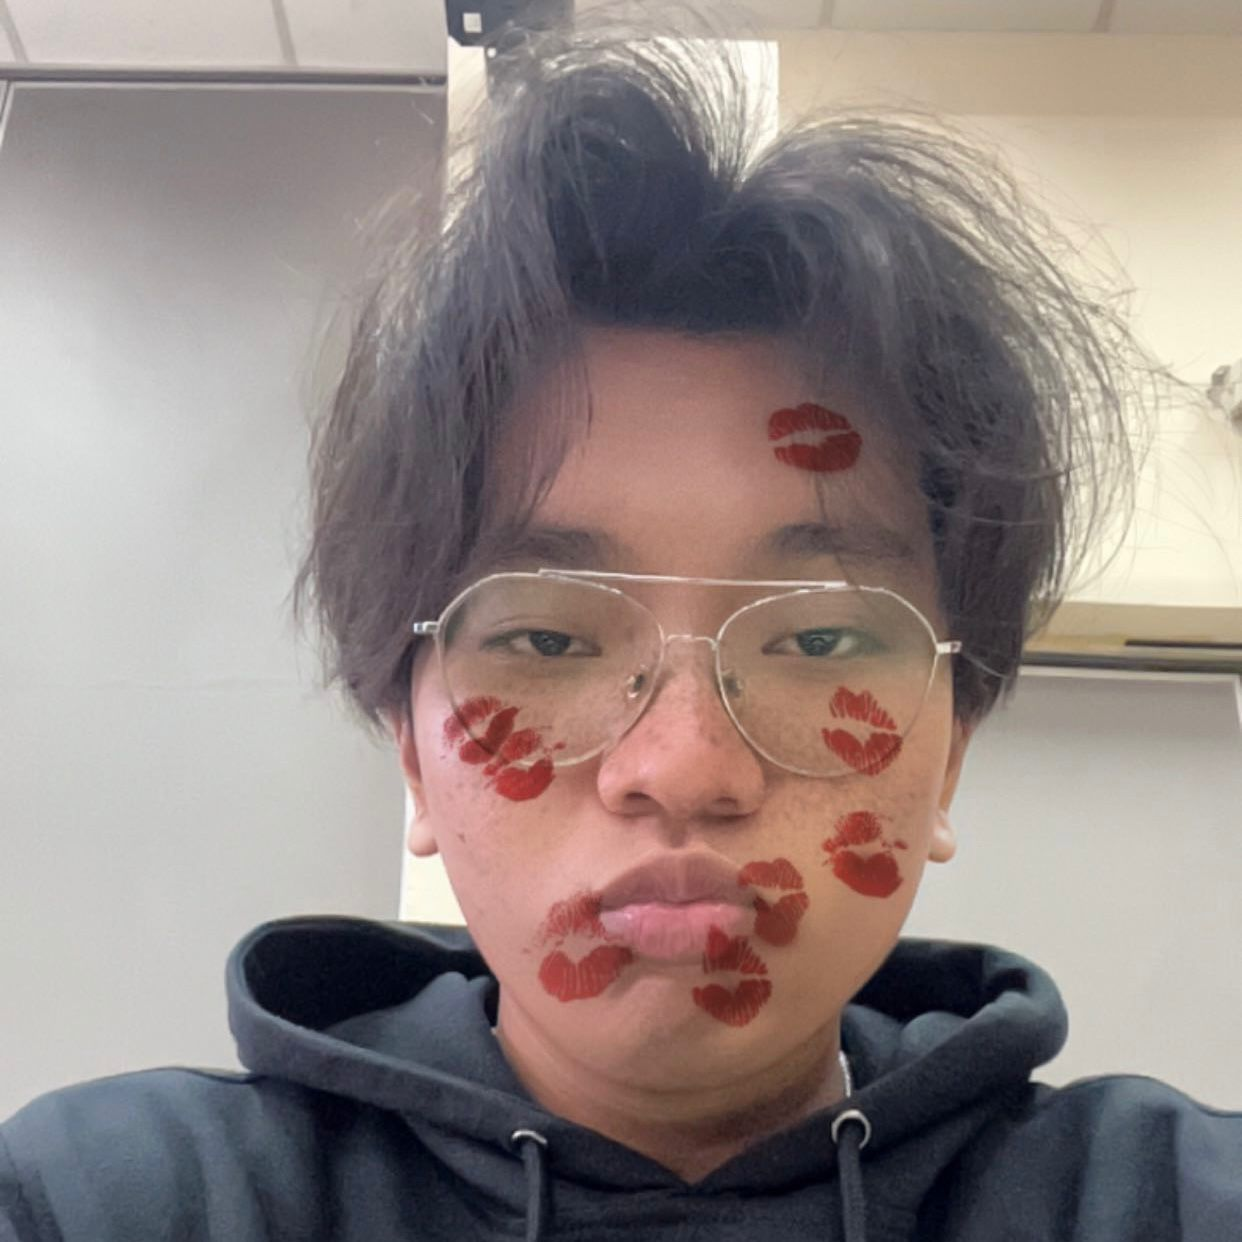
\includegraphics[width=9.5\linewidth,height=\textheight,keepaspectratio]{All_About_me/../images/ya.jpeg}

}

\caption{About Me}

\end{figure}%

Halo halo! Perkenalkan, saya Riantama Putra, mahasiswa Program Studi
Sistem dan Teknologi Informasi, Institut Teknologi Bandung, Angkatan
2024. Melalui tugas \emph{All About Me} ini, saya ingin mengenali diri
saya lebih dalam, bukan hanya sebagai mahasiswa, tetapi juga sebagai
pribadi yang sedang belajar memahami makna komunikasi, baik dengan diri
sendiri maupun dengan orang lain.

\section{Tentang Saya}\label{tentang-saya}

Saya melihat diri saya sebagai seseorang yang rasional tetapi tetap
hangat. Saya terbiasa berpikir dengan logika, namun tetap menghargai
sisi emosional dalam setiap interaksi. Dalam percakapan, saya lebih suka
mendengarkan terlebih dahulu dan mencoba memahami konteks sebelum
menanggapi. Namun, saya juga menyadari bahwa terkadang saya terlalu
berhati-hati, seolah takut dinilai salah. Dari sana saya belajar bahwa
komunikasi bukan soal menjadi sempurna, melainkan soal berani hadir apa
adanya dan mau memahami sebelum dipahami.

Saya percaya setiap orang memiliki cara unik untuk mengekspresikan diri.
Bagi saya, berbicara adalah proses untuk jujur terhadap diri sendiri,
dan mendengarkan adalah cara untuk memahami dunia dengan lebih luas.

\section{Nilai dan Prinsip yang Membentuk
Saya}\label{nilai-dan-prinsip-yang-membentuk-saya}

Dalam hidup, saya berpegang pada tiga hal: \textbf{kejujuran, empati,
dan tanggung jawab}. Kejujuran membuat saya bisa hidup tanpa
berpura-pura. Empati membantu saya memahami sudut pandang orang lain
tanpa langsung menghakimi. Dan tanggung jawab mengingatkan saya bahwa
setiap kata yang diucapkan membawa konsekuensi.

Dari perkuliahan ini, saya memahami bahwa nilai-nilai ini menjadi dasar
dalam \emph{self-concept} dan \emph{self-awareness}. Mengetahui siapa
diri saya dan apa yang saya hargai membantu saya berkomunikasi dengan
lebih sadar, terbuka, dan penuh tujuan. Saya juga belajar bahwa
mendengarkan dengan niat tulus dapat menciptakan hubungan yang lebih
bermakna dibanding sekadar berbicara panjang lebar.

\section{Cara Saya Melihat Dunia dan Orang
Lain}\label{cara-saya-melihat-dunia-dan-orang-lain}

Saya melihat dunia sebagai ruang untuk belajar. Tidak semua pelajaran
datang dari ruang kuliah, sebagian justru hadir lewat kesalahpahaman,
kegagalan, atau percakapan sederhana. Setiap kali saya berinteraksi,
saya berusaha untuk tidak hanya memahami kata-kata, tetapi juga perasaan
dan makna yang tersirat di baliknya.

Melalui teori komunikasi interpersonal, saya menyadari bahwa persepsi
sering kali menjadi sumber kesalahpahaman. Konflik tidak selalu muncul
karena niat buruk, tetapi karena perbedaan cara pandang. Karena itu,
saya mencoba menerapkan prinsip \textbf{``clarify before judge''} yang
memiliki arti mencari makna sebelum menyimpulkan. Pemahaman tentang
persepsi ini membantu saya mengurangi prasangka dan memperkuat
keterampilan empatik dalam berinteraksi.

\section{Kepribadian dan Kehidupan
Sehari-hari}\label{kepribadian-dan-kehidupan-sehari-hari}

Secara kepribadian, saya bisa dibilang cukup seimbang antara introvert
dan ekstrovert. Saya nyaman bekerja sendiri, tetapi juga menikmati waktu
bersama teman-teman yang punya energi positif. Di luar akademik, saya
menikmati hal-hal sederhana seperti mendengarkan musik, bermain game,
atau sekadar merenung sendiri. Momen-momen itu membantu saya memahami
diri saya dan mengatur emosi dengan lebih baik.

Saya belajar dari topik komunikasi nonverbal bahwa keheningan juga bisa
berbicara. Cara kita menatap, tersenyum, atau menunduk dapat
menyampaikan pesan tanpa kata-kata. Karena itu, saya mulai lebih sadar
terhadap bahasa tubuh saya dan mencoba menyesuaikannya agar selaras
dengan pesan yang ingin saya sampaikan.

\section{Refleksi atas Diri dan
Komunikasi}\label{refleksi-atas-diri-dan-komunikasi}

Selama mengikuti perkuliahan ini, saya belajar bahwa komunikasi sejati
berawal dari kesadaran diri (\emph{self-awareness}). Cara saya menilai
diri sendiri ternyata memengaruhi cara saya mendengar, memahami, dan
berbicara dengan orang lain. Saya belajar untuk tidak mencari penerimaan
dari semua orang (\emph{approval seeking}), tetapi untuk berbicara
dengan niat tulus dan menghargai perbedaan perspektif.

Saya juga mulai menerapkan \emph{affirmation}, yaitu berbicara baik
kepada diri sendiri. Satu kalimat positif kadang cukup untuk menenangkan
pikiran dan membantu saya menghadapi situasi sulit dengan kepala dingin.
Dari situ saya belajar bahwa komunikasi intrapersonal adalah pondasi
dari hubungan interpersonal yang sehat.

Dari materi \emph{Listening} saya menyadari pentingnya menjadi pendengar
aktif. Saya berusaha lebih fokus saat orang lain berbicara,
memparafrasekan untuk memastikan pemahaman saya benar, dan menghindari
kebiasaan \emph{pseudolistening}. Dengan mendengar sepenuhnya, saya
bukan hanya memahami pesan, tetapi juga menghargai manusia di baliknya.

\section{Harapan dan Tujuan ke Depan}\label{harapan-dan-tujuan-ke-depan}

Saya ingin menjadi pribadi yang tidak hanya cerdas secara teknis, tetapi
juga bijak dalam berinteraksi. Saya ingin kemampuan komunikasi saya
tidak berhenti pada penyampaian pesan, melainkan mampu membangun
kepercayaan dan kerja sama. Saya berharap dapat menciptakan lingkungan
yang terbuka, suportif, dan saling memahami, baik dalam konteks akademik
maupun profesional.

Bagi saya, komunikasi yang baik adalah cerminan kematangan diri.
\emph{All About Me} bukan sekadar tugas, tetapi proses belajar untuk
tumbuh menjadi pribadi yang memahami diri sendiri, mampu mendengarkan,
dan membawa nilai positif dalam setiap percakapan.

\begin{center}\rule{0.5\linewidth}{0.5pt}\end{center}

\begin{quote}
``Menjadi pendengar yang baik kadang lebih sulit daripada menjadi
pembicara yang hebat. Tetapi di sanalah kita belajar, bahwa memahami
orang lain selalu dimulai dari keberanian untuk mendengarkan.''
\end{quote}

\bookmarksetup{startatroot}

\chapter{UTS-2 My Songs for You}\label{uts-2-my-songs-for-you}

\textbf{Teruntuk Mia - Nuh\ldots{}}

\url{https://youtu.be/5j8pYsArkto?si=PZY8kkw47naUf03i}

Lagu ini saya pilih karena mewakili bentuk komunikasi yang lembut dan
tulus.\\
\emph{Teruntuk Mia} bukan hanya kisah tentang dua orang di bawah hujan,
tetapi juga tentang bagaimana perasaan bisa tersampaikan tanpa harus
dijelaskan secara panjang lebar.\\
Setiap nada dan baitnya mengingatkan saya bahwa komunikasi sejati tidak
selalu harus diucapkan, kadang cukup dirasakan.

Melalui lagu ini, saya belajar tentang \emph{komunikasi nonverbal},
bagaimana ekspresi, intonasi, dan suasana bisa menyampaikan pesan yang
lebih jujur daripada kata-kata.\\
Saya juga belajar bahwa mendengarkan lagu dengan hati membuat kita
berlatih \emph{empathy listening}, di mana kita berusaha memahami
perasaan di balik lirik, bukan sekadar mendengar melodi.

Lagu ini membantu saya merefleksikan \emph{self-awareness} saya sendiri,
tentang bagaimana saya mengekspresikan kasih, kehangatan, atau bahkan
kerinduan.\\
Seperti kata dosen di kelas, komunikasi interpersonal yang efektif
selalu dimulai dari kesadaran diri dan keberanian untuk hadir apa
adanya, tanpa topeng dan tanpa pura-pura.

\begin{center}\rule{0.5\linewidth}{0.5pt}\end{center}

\textbf{Lirik:}

\begin{longtable}[]{@{}
  >{\raggedright\arraybackslash}p{(\linewidth - 2\tabcolsep) * \real{0.5333}}
  >{\raggedright\arraybackslash}p{(\linewidth - 2\tabcolsep) * \real{0.4667}}@{}}
\toprule\noalign{}
\begin{minipage}[b]{\linewidth}\raggedright
Bagian
\end{minipage} & \begin{minipage}[b]{\linewidth}\raggedright
Lirik
\end{minipage} \\
\midrule\noalign{}
\endhead
\bottomrule\noalign{}
\endlastfoot
\textbf{Verse 1} & Berdua menunggu di sini Berharap hujan tak berhenti
Tetes demi tetes basahi Jalanan kota ini Dengan dirimu ku di sini
Sederhana tapi berarti Senyummu tetap melingkari Teduh tetap diberi \\
\textbf{Chorus} & Di antara senyumanmu Dan hujan di hari itu Aku tak
tahu mana yang lebih indah Di antara senyumanmu Dan hujan di hari itu
Aku tak tahu mana yang lebih indah \\
\textbf{Verse 2} & Berdua menunggu di sini Berharap hujan tak berhenti
Tetes demi tetes basahi Jalanan kota ini Dan ketika hujan t'lah mereda
Kita lanjutkanlah berjalan \\
\textbf{Instrumental Break} & \emph{Instrumen} \\
\textbf{Chorus} & Di antara senyumanmu Dan hujan di hari itu Aku tak
tahu mana yang lebih indah Di antara senyumanmu Dan hujan di hari itu
Aku tak tahu mana yang lebih indah \\
\textbf{Outro} & Aku tak tahu mana yang lebih indah \\
\end{longtable}

\bookmarksetup{startatroot}

\chapter{UTS-3 My Stories for You}\label{uts-3-my-stories-for-you}

\begin{figure}[H]

{\centering 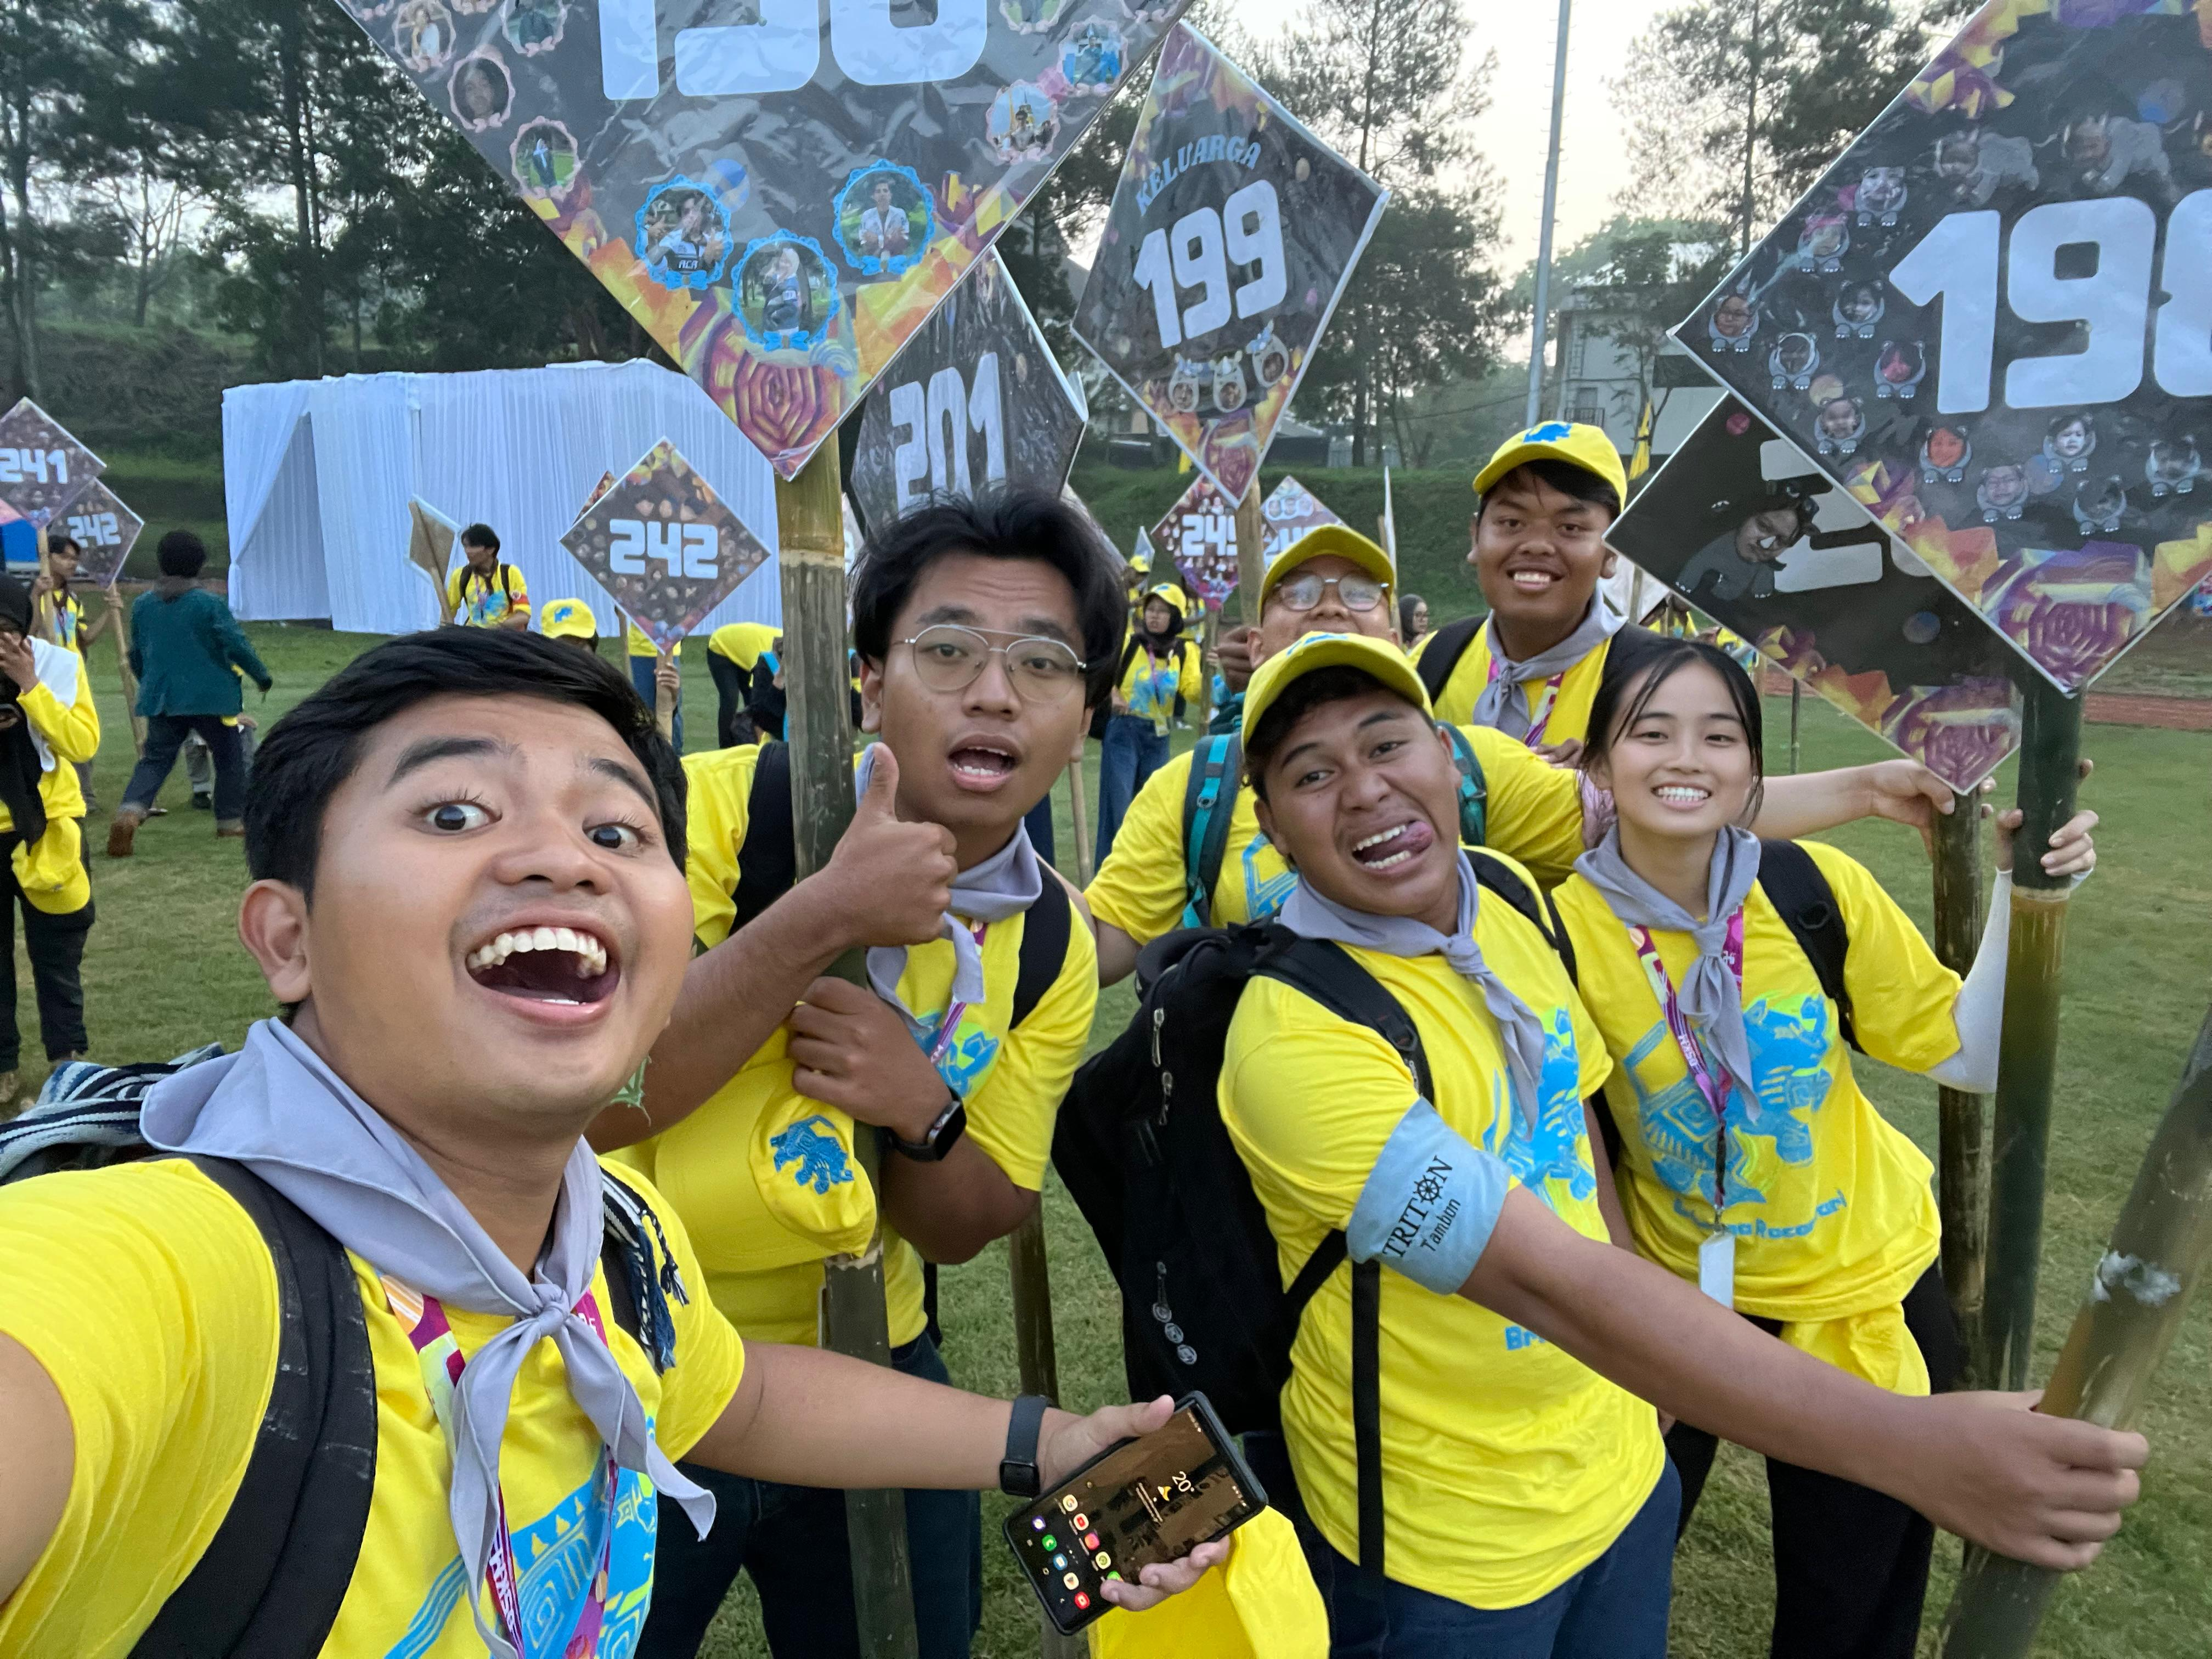
\includegraphics[width=9.5\linewidth,height=\textheight,keepaspectratio]{My_Stories_for_You/../images/oke.jpeg}

}

\caption{My Stories for You}

\end{figure}%

Menjadi mentor OSKM ITB 2025 adalah salah satu pengalaman paling
berharga dalam perjalanan saya sebagai mahasiswa.\\
Bukan hanya karena kesempatan untuk membimbing mahasiswa baru, tetapi
juga karena proses ini membuat saya belajar banyak tentang komunikasi,
empati, dan arti menjadi panutan yang sebenarnya.

\begin{center}\rule{0.5\linewidth}{0.5pt}\end{center}

\section{Awal Perjalanan dan
Motivasi}\label{awal-perjalanan-dan-motivasi}

Saya bergabung sebagai mentor karena ingin berkontribusi secara nyata
bagi lingkungan kampus.\\
Sejak awal, saya menyadari bahwa OSKM bukan sekadar acara penyambutan
mahasiswa baru, melainkan proses pembentukan karakter dan nilai
kebersamaan.\\
Saya ingin hadir di sana bukan sebagai ``pemberi nasihat,'' tetapi
sebagai teman yang mau mendengarkan, memahami, dan tumbuh bersama
mereka.

Motivasi ini muncul dari pengalaman pribadi.\\
Dulu, ketika saya menjadi peserta, ada satu mentor yang benar-benar
mendengarkan saya tanpa menghakimi.\\
Itu mengubah cara saya memandang peran seorang pembimbing.\\
Sejak saat itu, saya ingin melakukan hal yang sama --- menciptakan ruang
aman di mana orang bisa didengar dan merasa diterima.

\begin{center}\rule{0.5\linewidth}{0.5pt}\end{center}

\section{Proses dan Tantangan}\label{proses-dan-tantangan}

Menjadi mentor tidak semudah yang saya bayangkan.\\
Sejak tahap Sekolah Mentor, saya belajar bagaimana berkomunikasi dengan
berbagai tipe kepribadian.\\
Ada rekan mentor yang tegas, ada yang lembut, ada juga yang lebih
spontan.\\
Dari situ saya memahami bahwa komunikasi yang efektif bukan tentang
siapa yang paling banyak bicara, tapi siapa yang paling mampu
menyesuaikan diri.

Selama OSKM berlangsung, saya memegang satu kelompok mahasiswa baru.\\
Awalnya mereka pendiam dan agak canggung, tapi perlahan kehangatan mulai
tumbuh.\\
Saya belajar bahwa \emph{listening} adalah kunci untuk membangun
kedekatan.\\
Kadang mereka tidak butuh solusi, hanya butuh seseorang yang mau
mendengar tanpa menginterupsi.

Saya masih ingat satu malam saat salah satu peserta tiba-tiba
menghubungi saya lewat pesan pribadi.\\
Dia merasa tidak percaya diri karena belum terbiasa dengan lingkungan
kampus.\\
Saya membaca pesannya berkali-kali, mencoba memahami perasaannya lewat
pilihan kata dan nada tulisannya.\\
Saya menenangkan dia dengan bahasa yang sederhana dan jujur.\\
Esoknya, dia menyapa saya dengan senyum lebar --- tanpa perlu banyak
kata, saya tahu komunikasi kami berhasil.

\begin{center}\rule{0.5\linewidth}{0.5pt}\end{center}

\section{Pembelajaran dan Refleksi}\label{pembelajaran-dan-refleksi}

Dari pengalaman menjadi mentor, saya menyadari bahwa komunikasi bukan
sekadar menyampaikan pesan, tapi juga membangun hubungan yang
bermakna.\\
Saya belajar bahwa bahasa tubuh, intonasi, dan tatapan mata bisa
berbicara lebih jujur daripada kalimat panjang.\\
Saya juga belajar mengelola persepsi: memahami kapan harus tegas, dan
kapan harus lembut.

Yang paling berkesan bagi saya adalah bagaimana saya ikut tumbuh bersama
para peserta.\\
Saya yang awalnya ragu untuk memimpin kini lebih berani untuk berbicara,
mendengar, dan mengarahkan tanpa harus memaksa.\\
Saya belajar untuk tidak hanya memahami teori komunikasi, tetapi
benar-benar mempraktikkannya dalam konteks sosial yang nyata.

Menjadi mentor juga mengajarkan saya tentang empati --- untuk melihat
sesuatu dari sudut pandang orang lain tanpa tergesa-gesa menilai.\\
Ketika saya mulai benar-benar mendengarkan, saya menyadari bahwa setiap
individu membawa cerita dan perjuangannya sendiri.

\begin{center}\rule{0.5\linewidth}{0.5pt}\end{center}

\section{Penutup}\label{penutup}

Menjadi mentor OSKM bukan hanya tentang memimpin, tetapi tentang belajar
memahami.\\
Saya belajar bahwa setiap interaksi memiliki makna, setiap percakapan
adalah kesempatan untuk menumbuhkan kepercayaan, dan setiap diam pun
punya arti jika kita mau mendengarkan dengan hati.

Saya merasa bangga bisa menjadi bagian dari proses ini.\\
Karena di balik setiap kegiatan dan percakapan kecil, ada pelajaran
besar tentang tanggung jawab, komunikasi, dan kemanusiaan.\\
Dan bagi saya, itulah inti dari menjadi seorang mentor.

\bookmarksetup{startatroot}

\chapter{UTS-4 My SHAPE (Spiritual Gifts, Heart, Abilities, Personality,
Experiences)}\label{uts-4-my-shape-spiritual-gifts-heart-abilities-personality-experiences}

Halaman ini merupakan refleksi pribadi yang membantu saya memahami siapa
diri saya secara utuh.\\
Melalui lima dimensi \textbf{SHAPE} (Strengths, Heart, Aptitudes,
Personality, dan Experiences), saya mencoba mengenali pola unik yang
membentuk cara saya berpikir, bertindak, dan berkontribusi dalam
kehidupan akademik maupun sosial.

\begin{center}\rule{0.5\linewidth}{0.5pt}\end{center}

\section{S - Signature Strengths (Kekuatan
Khas)}\label{s---signature-strengths-kekuatan-khas}

\textbf{Love of Learning}\\
Saya memiliki rasa ingin tahu yang tinggi terhadap hal-hal baru. Saya
menikmati proses belajar, bukan hanya hasil akhirnya. Saat menghadapi
konsep yang sulit, saya tertarik untuk mencari tahu hingga benar-benar
memahami maknanya. Kekuatan ini membuat saya adaptif dalam berbagai
situasi, baik di perkuliahan maupun dalam organisasi.

\textbf{Kindness}\\
Saya percaya bahwa kebaikan adalah bahasa komunikasi yang universal.
Dalam tim atau lingkungan sosial, saya berusaha menjaga suasana agar
tetap positif dan saling menghargai. Saya merasa paling hidup ketika
bisa membuat orang lain merasa dimengerti, terutama melalui sikap
mendengarkan dan empati.

\textbf{Leadership}\\
Saya cenderung mengambil inisiatif ketika dibutuhkan dan berusaha
membimbing rekan-rekan agar tujuan bersama tercapai. Bagi saya,
kepemimpinan bukan tentang memerintah, tetapi tentang memberi arah,
menenangkan suasana, dan membantu orang lain berkembang bersama.

\begin{center}\rule{0.5\linewidth}{0.5pt}\end{center}

\section{H - Heart (Nilai dan Gairah)}\label{h---heart-nilai-dan-gairah}

\textbf{Empati dan Kepedulian}\\
Saya merasa terdorong ketika bisa membantu orang lain tumbuh. Dalam
kegiatan mentoring dan proyek kelompok, saya belajar bahwa keberhasilan
bersama lebih bermakna daripada pencapaian individu. Saya ingin menjadi
seseorang yang membawa semangat kolaborasi dan saling pengertian.

\textbf{Komunikasi dan Pengembangan Diri}\\
Saya memiliki minat besar pada dunia komunikasi interpersonal. Bagi
saya, berbicara dan mendengarkan bukan sekadar bertukar kata, tetapi
juga membangun makna dan kepercayaan. Saya selalu berusaha mengasah
kemampuan ini agar dapat berkomunikasi dengan lebih sadar dan reflektif.

\textbf{Teknologi untuk Kemanusiaan}\\
Sebagai mahasiswa Sistem dan Teknologi Informasi, saya tertarik pada
bagaimana teknologi bisa digunakan untuk membantu manusia, bukan
menggantikannya. Saya percaya bahwa sistem yang baik adalah yang mampu
memahami kebutuhan manusia secara empatik.

\begin{center}\rule{0.5\linewidth}{0.5pt}\end{center}

\section{A - Aptitudes \& Acquired Skills (Bakat dan
Keterampilan)}\label{a---aptitudes-acquired-skills-bakat-dan-keterampilan}

\textbf{Hard Skills}\\
1. Pemrograman (Python, HTML, CSS, JavaScript)\\
2. Pengolahan dan visualisasi data\\
3. Desain komunikasi menggunakan Canva dan Photoshop\\
4. Editing video dan konten media digital

\textbf{Soft Skills}\\
1. Komunikasi efektif dan mendengarkan aktif\\
2. Kepemimpinan dan manajemen waktu\\
3. Kolaborasi tim dan penyelesaian masalah\\
4. Adaptabilitas dan berpikir reflektif

Saya menyadari bahwa keterampilan bukan sekadar alat, tetapi cerminan
dari karakter.\\
Keterampilan teknis membantu saya berpikir sistematis, sementara
keterampilan interpersonal menjaga saya tetap manusiawi dalam setiap
prosesnya.

\begin{center}\rule{0.5\linewidth}{0.5pt}\end{center}

\section{P - Personality
(Kepribadian)}\label{p---personality-kepribadian}

Saya termasuk tipe \textbf{ENFJ -- The Protagonist}, pribadi yang
cenderung hangat, visioner, dan senang membantu orang lain menemukan
potensinya. Saya merasa nyaman berada di lingkungan yang dinamis, di
mana setiap orang bisa berkembang bersama.

Saya menyukai keteraturan, tapi juga terbuka terhadap perubahan. Ketika
berinteraksi, saya berusaha menyeimbangkan logika dengan empati, karena
saya percaya bahwa keputusan yang baik adalah keputusan yang tidak hanya
benar secara rasional, tetapi juga bijak secara emosional.

Bagi saya, kepribadian bukan sesuatu yang membatasi, melainkan fondasi
untuk terus belajar menyesuaikan diri.

\begin{center}\rule{0.5\linewidth}{0.5pt}\end{center}

\section{E - Experiences (Pengalaman dan Pelajaran
Hidup)}\label{e---experiences-pengalaman-dan-pelajaran-hidup}

Pengalaman yang paling berpengaruh bagi saya adalah ketika menjadi
\textbf{mentor OSKM ITB 2025}.\\
Dalam peran itu, saya belajar banyak tentang komunikasi yang sejati.
Tidak semua peserta datang dengan semangat yang sama, dan tidak semua
cerita bisa dijawab dengan kata-kata.\\
Terkadang, mereka hanya butuh seseorang yang benar-benar mendengarkan
tanpa menghakimi.

Saya belajar bahwa \emph{presence} adalah bentuk komunikasi yang paling
jujur.\\
Dari situ saya memahami bahwa menjadi mentor bukan hanya tentang
memimpin, tetapi juga tentang melayani, memahami, dan membangun ruang
aman bagi orang lain untuk tumbuh.

Selain itu, pengalaman bekerja dalam tim lintas latar belakang membuat
saya belajar pentingnya persepsi dan kesadaran kontekstual.\\
Bahwa setiap orang memaknai pesan dengan cara berbeda, dan tugas kita
adalah menjembatani perbedaan itu dengan empati.

\begin{center}\rule{0.5\linewidth}{0.5pt}\end{center}

\section{My Personal Mission
Statement}\label{my-personal-mission-statement}

``Menjadi pribadi yang hadir dengan kesadaran penuh, menggunakan
kemampuan berpikir dan empati untuk membantu orang lain berkembang,
serta menciptakan lingkungan yang manusiawi dalam setiap interaksi.''

Misi ini menjadi pengingat bagi saya untuk tidak hanya berfokus pada
pencapaian pribadi, tetapi juga pada nilai dan dampak dari setiap
langkah yang saya ambil.

\begin{center}\rule{0.5\linewidth}{0.5pt}\end{center}

\section{Refleksi Akhir}\label{refleksi-akhir}

Menulis \emph{My SHAPE} membuat saya menyadari bahwa diri saya tidak
hanya dibentuk oleh kemampuan dan pencapaian, tetapi juga oleh nilai,
pengalaman, dan hubungan dengan orang lain.\\
Saya belajar bahwa mengenal diri adalah perjalanan yang tidak pernah
selesai, karena manusia terus bertumbuh dari setiap interaksi dan
pengalaman baru.

Saya semakin memahami bahwa komunikasi bukan hanya keterampilan, tetapi
cara kita menghargai eksistensi orang lain.\\
Setiap kata yang diucapkan, setiap diam yang dipilih, adalah bagian dari
proses memahami --- baik diri sendiri maupun sesama.

\begin{quote}
``Ketika kita benar-benar memahami diri, kita akan tahu bagaimana
seharusnya hadir untuk orang lain.''
\end{quote}

\bookmarksetup{startatroot}

\chapter{UTS-5 My Personal Reviews}\label{uts-5-my-personal-reviews}

\section{Identifikasi}\label{identifikasi}

\begin{itemize}
\tightlist
\item
  \textbf{Nama \& NIM:} Riantama Putra -- 18224061\\
\item
  \textbf{Penilai:} Self-assessment (Riantama Putra)\\
\item
  \textbf{Cakupan:} Portofolio UTS (UTS-1 s.d. UTS-5) pada situs
  \href{https://veinsan.github.io/all-about-me/}{ii-2100.github.io/all-about-me}
\end{itemize}

\begin{center}\rule{0.5\linewidth}{0.5pt}\end{center}

\section{Tinjauan Umum}\label{tinjauan-umum}

Portofolio ini berisi rangkaian refleksi diri yang mencerminkan proses
pembelajaran komunikasi interpersonal saya selama setengah semester.\\
Setiap bagian memiliki fokus berbeda:

\begin{itemize}
\tightlist
\item
  \textbf{UTS-1 (All About Me)} menampilkan identitas dan nilai
  personal,\\
\item
  \textbf{UTS-2 (My Songs for You)} mengekspresikan pesan emosional
  melalui karya musik,\\
\item
  \textbf{UTS-3 (My Stories for You)} merefleksikan pengalaman
  interpersonal dan nilai kemanusiaan,\\
\item
  \textbf{UTS-4 (My SHAPE)} menjabarkan hasil asesmen diri berdasarkan
  VIA dan SHAPE,\\
\item
  \textbf{UTS-5 (My Personal Reviews)} adalah telaah kritis terhadap
  seluruh karya di atas.
\end{itemize}

Secara umum, kekuatan utama dari portofolio ini terletak pada kejujuran
reflektif, keterhubungan antara teori dan pengalaman nyata, serta
konsistensi nada personal dalam penulisan.\\
Area yang masih bisa dikembangkan adalah kedalaman analisis dan
kejelasan rekomendasi berbasis konsep komunikasi interpersonal.

\begin{center}\rule{0.5\linewidth}{0.5pt}\end{center}

\section{Tinjauan Spesifik dan Skor}\label{tinjauan-spesifik-dan-skor}

\subsection{UTS-1 --- All About Me}\label{uts-1-all-about-me-1}

\textbf{Skor:} Orisinalitas 4, Keterlibatan 4, Humor 2, Wawasan 5 →
\textbf{15/20 (75\%)}\\
Tulisan ini menggambarkan kesadaran diri dengan baik, menyertakan nilai
dan prinsip pribadi yang konsisten.\\
Masih bisa diperkuat dengan pembuka yang lebih menggugah secara naratif
agar pembaca langsung terhubung secara emosional.

\textbf{Rekomendasi:} Tambahkan cerita kecil atau pengalaman reflektif
sebagai pengantar untuk menonjolkan keunikan diri.

\begin{center}\rule{0.5\linewidth}{0.5pt}\end{center}

\subsection{UTS-2 --- My Songs for You}\label{uts-2-my-songs-for-you-1}

\textbf{Skor:} Orisinalitas 4, Keterlibatan 4, Humor 2, Inspirasi 4 →
\textbf{14/20 (70\%)}\\
Pemilihan lagu ``Teruntuk Mia'' menghadirkan pesan interpersonal yang
puitis dan hangat.\\
Kekuatan terletak pada kesederhanaan makna dan kejujuran emosi.\\
Masih bisa diperkuat dengan refleksi singkat tentang hubungan antara
lirik dan nilai komunikasi interpersonal seperti empati dan persepsi
makna.

\textbf{Rekomendasi:} Tambahkan paragraf interpretasi pribadi tentang
lagu tersebut, terutama bagaimana lagu itu mencerminkan \emph{presence}
dan \emph{emotional expression}.

\begin{center}\rule{0.5\linewidth}{0.5pt}\end{center}

\subsection{UTS-3 --- My Stories for
You}\label{uts-3-my-stories-for-you-1}

\textbf{Skor:} Orisinalitas 5, Keterlibatan 5, Pengembangan 5, Inspirasi
5 → \textbf{20/20 (100\%)}\\
Kisah menjadi mentor OSKM ITB 2025 sangat kuat, otentik, dan
inspiratif.\\
Tulisan ini menggambarkan dinamika interpersonal, empati, dan refleksi
diri dengan mendalam.\\
Struktur naratifnya mengalir alami dan menunjukkan pemahaman nyata
terhadap konsep komunikasi efektif dan kesadaran sosial.

\textbf{Rekomendasi:} Cerita sudah sangat matang; bisa ditambah satu
paragraf penutup yang mengaitkan pengalaman dengan teori ``self and
others'' dari materi kuliah minggu ke-3.

\begin{center}\rule{0.5\linewidth}{0.5pt}\end{center}

\subsection{UTS-4 --- My SHAPE}\label{uts-4-my-shape}

\textbf{Skor:} Orisinalitas 5, Keterlibatan 5, Pengembangan 5, Inspirasi
4 → \textbf{19/20 (95\%)}\\
Isi halaman menggambarkan analisis diri yang utuh dan integratif.\\
Tiap elemen SHAPE (Strengths, Heart, Aptitudes, Personality,
Experiences) dijabarkan dengan jelas dan reflektif.\\
Refleksi personal di bagian akhir menguatkan kesadaran terhadap peran
diri dalam komunikasi interpersonal.

\textbf{Rekomendasi:} Bisa ditambahkan tabel singkat rekap hasil asesmen
VIA agar pembaca langsung melihat data pendukung kekuatan diri.

\begin{center}\rule{0.5\linewidth}{0.5pt}\end{center}

\subsection{UTS-5 --- My Personal
Reviews}\label{uts-5-my-personal-reviews-1}

\textbf{Skor:} Pemahaman Konsep 5, Analisis Kritis 5, Argumentasi 4,
Etos \& Empati 5, Rekomendasi 4 → \textbf{23/25 (92\%)}\\
Bagian ini menampilkan pemahaman menyeluruh terhadap konsep komunikasi
interpersonal.\\
Analisisnya logis, runtut, dan mengaitkan teori dengan praktik
reflektif.\\
Gaya penulisan menunjukkan empati dan kedewasaan berpikir, dengan saran
yang konkret dan aplikatif.

\textbf{Rekomendasi:} Tambahkan satu kalimat pembuka yang menjelaskan
pentingnya melakukan \emph{self-review} sebagai bagian dari komunikasi
reflektif diri.

\begin{center}\rule{0.5\linewidth}{0.5pt}\end{center}

\section{Rekap Nilai}\label{rekap-nilai}

\begin{longtable}[]{@{}lll@{}}
\toprule\noalign{}
Tugas & Skor & Persentase \\
\midrule\noalign{}
\endhead
\bottomrule\noalign{}
\endlastfoot
UTS-1 & 15/20 & 75\% \\
UTS-2 & 14/20 & 70\% \\
UTS-3 & 20/20 & 100\% \\
UTS-4 & 19/20 & 95\% \\
UTS-5 & 23/25 & 92\% \\
\end{longtable}

\textbf{Rata-rata total:} 90.4\% → \emph{Sangat Baik (A)}

\begin{center}\rule{0.5\linewidth}{0.5pt}\end{center}

\section{Refleksi Akhir}\label{refleksi-akhir-1}

Melalui proses \emph{self-assessment} ini, saya belajar bahwa refleksi
bukan sekadar menilai hasil, tetapi meninjau kembali proses berpikir,
perasaan, dan interaksi yang saya alami.\\
Saya menyadari bahwa komunikasi interpersonal tidak bisa dilepaskan dari
kesadaran diri dan empati.\\
Menilai diri sendiri dengan jujur membantu saya memahami bagaimana saya
belajar, berinteraksi, dan berkembang.

Mata kuliah ini bukan hanya memberi teori, tetapi juga ruang untuk
mengenal siapa saya dalam konteks sosial dan emosional.\\
Saya berharap pemahaman ini bisa terus saya bawa ke kehidupan
profesional, agar komunikasi saya selalu jujur, hangat, dan bermakna.

\begin{quote}
``Menilai diri sendiri dengan jujur adalah langkah pertama untuk tumbuh
menjadi pribadi yang lebih memahami orang lain.''
\end{quote}

\bookmarksetup{startatroot}

\chapter{UAS-1 My Concepts}\label{uas-1-my-concepts}

Mau hidup epik ? \href{lifestory.pdf}{Write your Life Story}

Apa itu berkonsep?

\url{https://youtu.be/QVfUlVBO80U?si=yM6q_rwV9rcDBbu7}

\bookmarksetup{startatroot}

\chapter{UAS-3 My Opinions}\label{uas-3-my-opinions}

SApa itu beropini? \href{BM\%20Opini.mp4}{Opini Berpengaruh}

Bagiamana menjaadi menarik? \href{./Interesting.mp4}{Menjadi Menarik}

\bookmarksetup{startatroot}

\chapter{UAS-3 My Innovations}\label{uas-3-my-innovations}

\bookmarksetup{startatroot}

\chapter{UAS-4 My Knowledge}\label{uas-4-my-knowledge}

Cara saya mengkomunikasikan sebuah pengatahuan sebagai petunjuk bagi
orang lain 1) saya tulis
\href{Rekomendasi\%20Presentasi\%20Efektif(Contoh\%20Makalah).pdf}{makalah
sebagai bahan utama} 2) lalu saya buat
\href{Contoh\%20Transkrip\%20Presentasi.pdf}{transkrip ucapan lisan} 3)
kemudian saya kembangkan
\href{Rekomendasi\%20Presentasi\%20(Contoh\%20Slides).pdf}{slide
pendukung trnsskrip} 4) lalu saya memproduksivideo audio visual
\url{https://youtu.be/ZbghfMvnPZc} \url{https://youtu.be/ZbghfMvnPZc}

\bookmarksetup{startatroot}

\chapter{UAS-5 My Professional
Reviews}\label{uas-5-my-professional-reviews}

Untuk melAkukan review, seperti pada
\href{../My_Personal_Reviews/Doc.5.Mengevaluasi-Esai-Berdasarkan-Rubrik.pdf}{pendekatan
AI}, kita membutuhkan rubrik

\bookmarksetup{startatroot}

\chapter{Summary}\label{summary}

In summary, this book has no content whatsoever.

\bookmarksetup{startatroot}

\chapter*{References}\label{references}
\addcontentsline{toc}{chapter}{References}

\markboth{References}{References}

\phantomsection\label{refs}




\end{document}
